%% question-12.tex
%%

%% ==============================
\subsection{Modélisation explicite d'une expression}
\label{sec:question12}
%% ==============================

Le concept d'expression est présenté à l'aide de la figure \ref{fig:expression}. Une \emph{Expression} contient une \emph{Parenthese} et peut prendre la forme de celle-ci. Une Expression peut aussi être un \emph{Literal} qui est une variable, une 
\emph{ExpressionGauche} qui elle même peut être un \emph{AppelVariable} qui invoque une variable, un \emph{AppelChamp} qui provient d'un \emph{Enregistrement}, un \emph{AppelCellule} qui a comme source un \emph{Tableau}. Une \emph{Expression} peut aussi être
un \emph{AppelModule} comportant des \emph{Parametre}, une \emph{Expression Unaire} ou \emph{Binaire} comportant des \emph{Operateur}.

\begin{figure}
	\centering
	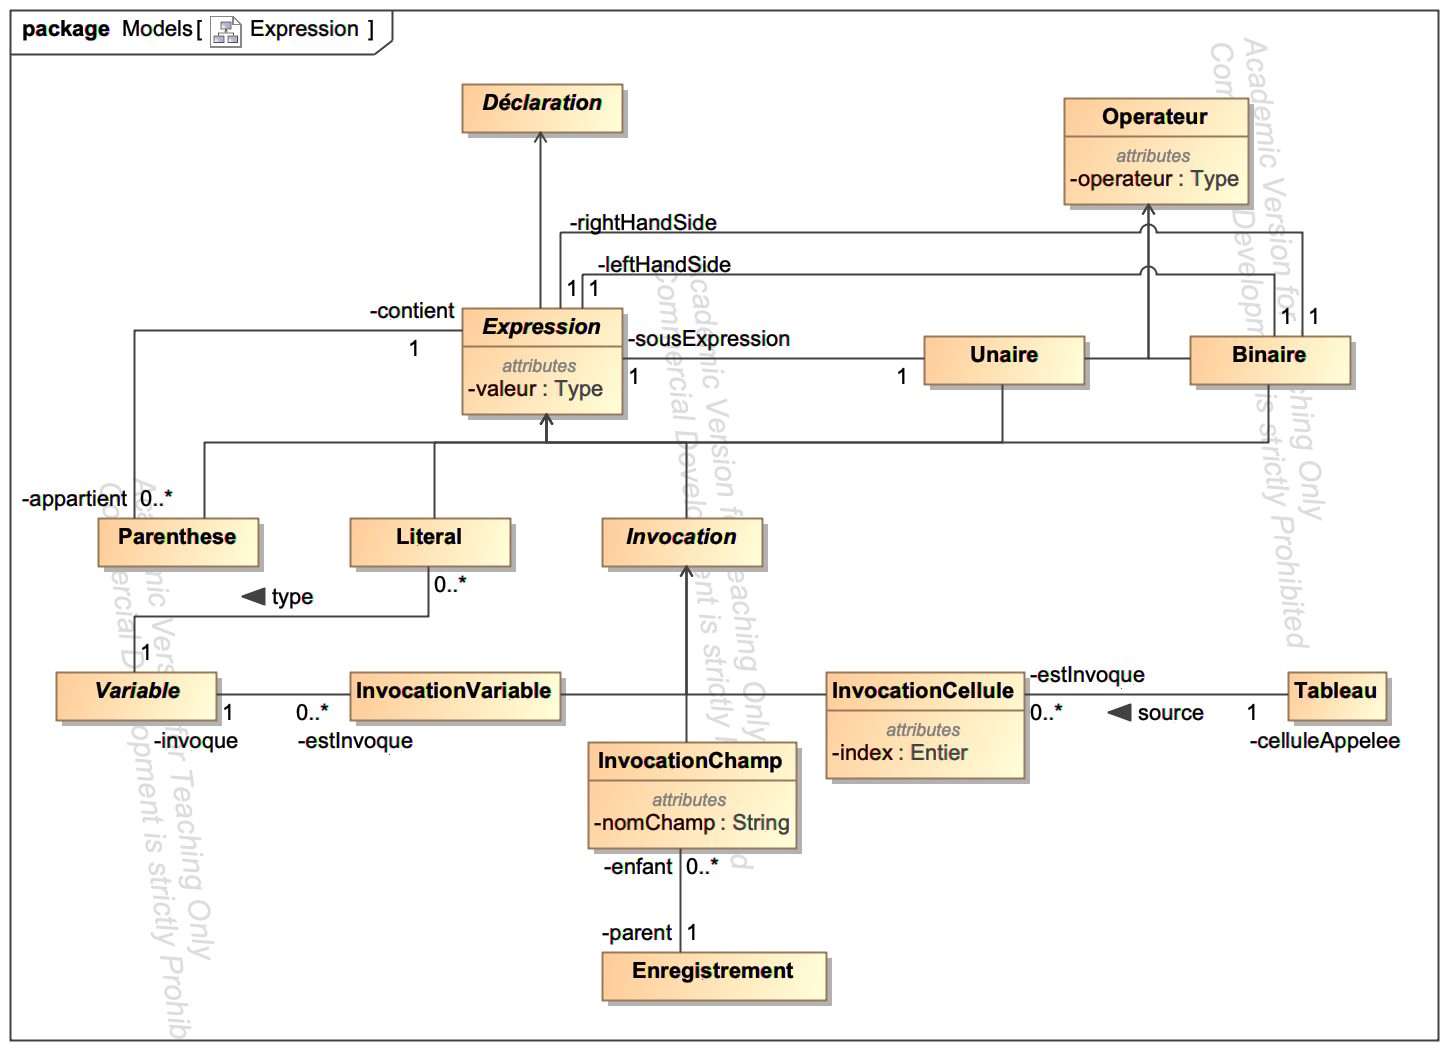
\includegraphics[width=500pt]{assets/class__Expression}
	\caption{Diagramme de classe d'une expression}
	\label{fig:expression}
\end{figure}